\documentclass{article}
\usepackage[
top    = 2.75cm,
bottom = 2.50cm,
left   = 3.00cm,
right  = 2.50cm]{geometry}
\usepackage{hyperref}
\usepackage{cite}
\usepackage{setspace}
\usepackage{algorithm}
\usepackage{graphicx}
\graphicspath{ {./images/} }
\title{\vspace{-2.0cm} A Generalizable Framework for Automated Cloud Configuration Selection \\ \vspace{0.5cm} \large Supervisors: Adam Barker \& Yuhui Lin}
\date{2019-06-06}
\author{Jack Briggs - 140011358 \\ MSc Data-Intensive Analysis}
\doublespacing
\begin{document}

\section*{Evaluation}
To demonstrate the effectiveness of the implementation of our framework, we wanted to show that it could replicate the methods set out in the Cherrypick paper \cite{Alipourfard2017} by performing Bayesian Optimization to attempt to find an optimal configuration for a given deployment. We then wanted to use the same implementation to perform multiple exhaustive searches so that the results from Bayesian Optimization could be properly compared to the real average results.

\paragraph{}
Video streaming is one of the most common services for which cloud servers are used, where video files are transcoded to an appropriate file type and streamed to an end-user's device\cite{JunXin2005, Lottarini2018}.
The deployment to be used was originally planned to be Cloudsuite3's media streaming benchmark\cite{Palit2016}, however this was found to be extremely variable and dependent entirely on network bandwidth, and so instead the vBench video transcoding benchmark was used\cite{Lottarini2018}. Our objective function measured an instance type's relative rate of transcoding of a single 5 second 1920x1080 video file, returning a score of 0 if the quality was below a given threshold, divided by the hourly price of that instance. Effectively, we maximised the rate of transcoding a unit of video length at a sufficient quality per hourly cost. We had hoped to show that incorporating the soft constraint on video quality within the value returned by the Interpreter, rather than within the Acquisition function as was done in Cherrypick, did not hinder the optimization process, however no instance type tested failed to achieve the threshold video quality in any case.

\paragraph{}
For choosing the boundaries of the search space, we decided to reduce costs by using only machines ranging from 2 vCPUs to 8 vCPUs. This was also convenient as to use more powerful machines would have required requesting additional raised quotas from the providers used, and so would be less easily replicable by others wishing to repeat our evaluation. As we wanted to show that the implementation worked with multiple providers, and were were ensuring our input variables matched exactly to an available instance type, we could not rely on Google cloud platform's custom machine types and had to find some way to categorize possible variables. Rather than including memory as a variable, CPU instead was coded as a categorical variable (2, 4, or 8), along with machine category (General, Memory, CPU), each with a different amount of memory. Table \ref{tab:instance-types} show which machine types corresponded to each option. 

\begin{table}[!hb]
\centering
\begin{tabular}{ |c||c|c|  }
 \hline
 & \multicolumn{2}{|c|}{Provider} \\
 \hline
 Machine Category & Amazon EC2 & Google Compute Engine \\
 \hline
 General& n1-standard & m5\\
 Memory & n1-highmem  & r5\\
 CPU    & n1-highcpu  & c5\\
 \hline
\end{tabular}
\caption{Machine types corresponding to different instance categories for the two providers}
\label{tab:instance-types}
\end{table}

For more resource-intensive situations, the search space could follow this same pattern, with the CPU variable extended, possibly instead as an integer between 1 and 6 which 2 is raised to the power of to determine vCPU number, as this covers many of the available CPU options.

The 18 machine types decided upon (3 vCPU numbers for 3 machine categories for the 2 providers) were stored in a single CSV dataset for use with the instance Selector. A vBench Deployer was used which utilized Terraform to provision a single instance of the given machine type, on which the remote docker API was used to deploy and collect logs from an docker image containing vBench. An Interpreter then isolated the vBench score from these logs, and divided it by the hourly cost of that machine type to return the final value.

Where not otherwise specified, statistical results are quoting the p-values returned from a Tukey's Honest Significant differences test to correct for multiple comparisons. Analysis was performed in RStudio\cite{R, RStudio}, and full logs as well and scripts used for analysis are available on the project's Github repository.

\paragraph{}
The results of the exhaustive search are shown in figures \ref{fig:vBench-scores} and \ref{fig:vBench-values}. The raw scores (time taken to transcode relative to the reference) show clear overlap between many possible configurations. While in general they show a significant difference between 2 vCPUs and either 4 ($P < .001$) or 8 ($P < .001$) vCPUs, where the score increases with vCPU number, they show less certain differences between 4 and 8 ($P = .066$), dependent on the provider and machine category, suggesting either diminishing returns or a limit of the benchmark to utilize all vCPU cores.
 
\begin{figure}
  \centering
   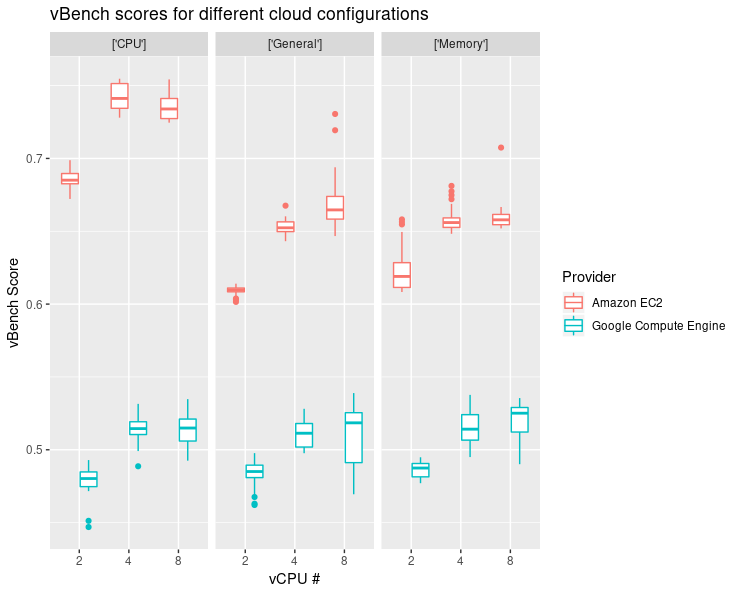
\includegraphics[scale=0.8]{vbench_scores}
   \caption{Distribution of vBench scores}
  \label{fig:vBench-scores}
\end{figure}
\begin{figure}
  \centering
   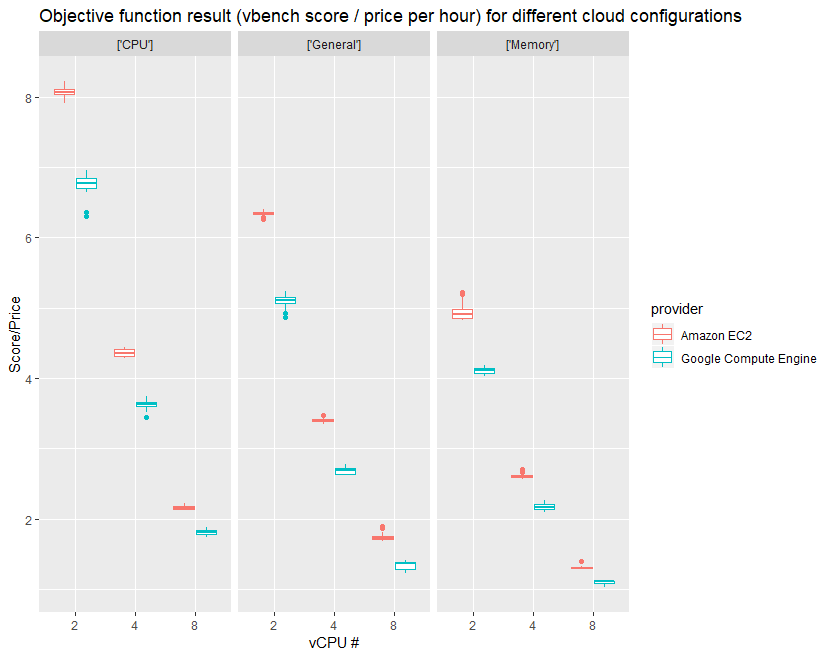
\includegraphics[scale=0.8]{vbench_values}
   \caption{Distribution of objective function values}
  \label{fig:vBench-values}
\end{figure}
\begin{figure}
  \centering
  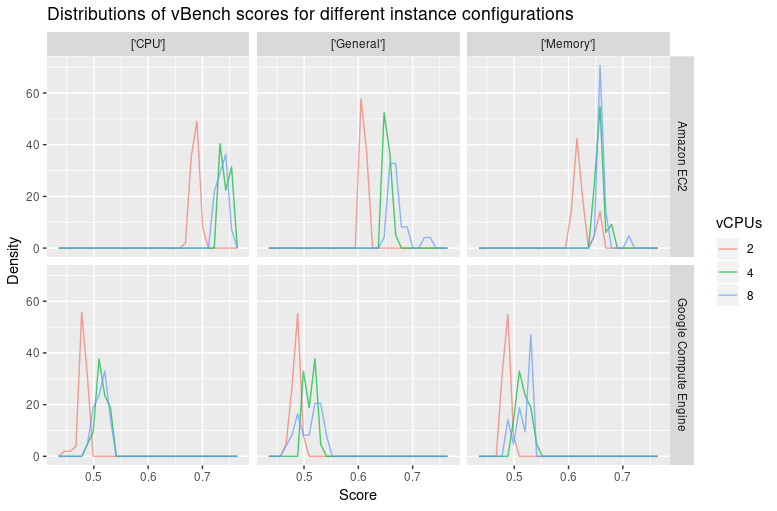
\includegraphics[scale=0.7]{vbench_dists}
  \caption{Distribution of vBench scores in frequency polygons}
  \label{fig:vBench-dists}
\end{figure}

However, once the scores are divided by that machine's hourly costs, there is much less overlap. A clear optimal configuration can be seen in the c5.large machine type, if one is purely interested in getting the most video transcoding for a given cost. The c5.large machine was significantly better than the next best option, the n1-highcpu-2 ($P < .001$). Amazon EC2's  machine types consistently outperformed Google Compute Engine's equivalents of the same category and vCPU number at both raw score (Anova, $F = 32111.456, P < .001$) and value for money (Anova, $F = 22710.7, P < .001$). However, despite this general trend, the provider seemed to be the least important factor in determining the optimal configuration. For example, the n1-highcpu-2 still gave significantly better values than the m5.large ($P < .001$), or the c5.xlarge ($P < .001$) making it the second most cost-efficient option. 

\begin{figure}
  \caption{Optimal configurations suggested after convergence for Bayesian Optimization searches}
  \label{fig:bo-results}
  \centering
  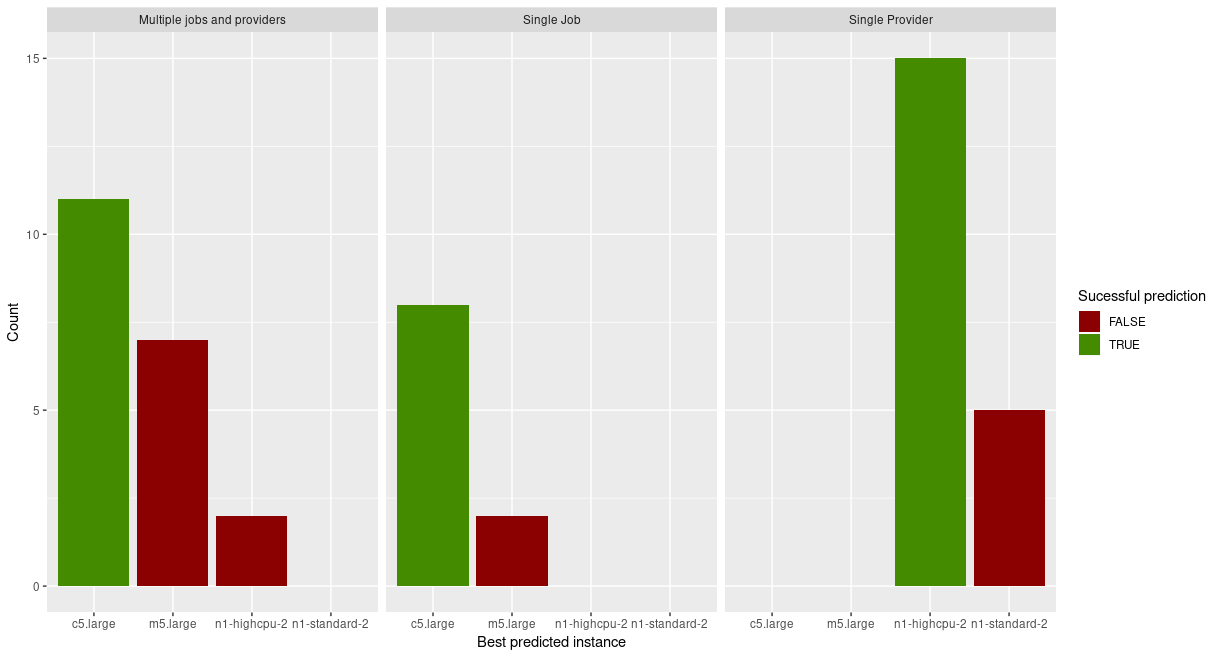
\includegraphics[scale=0.5]{bo_results}
\end{figure}
\begin{figure}
	\centering
	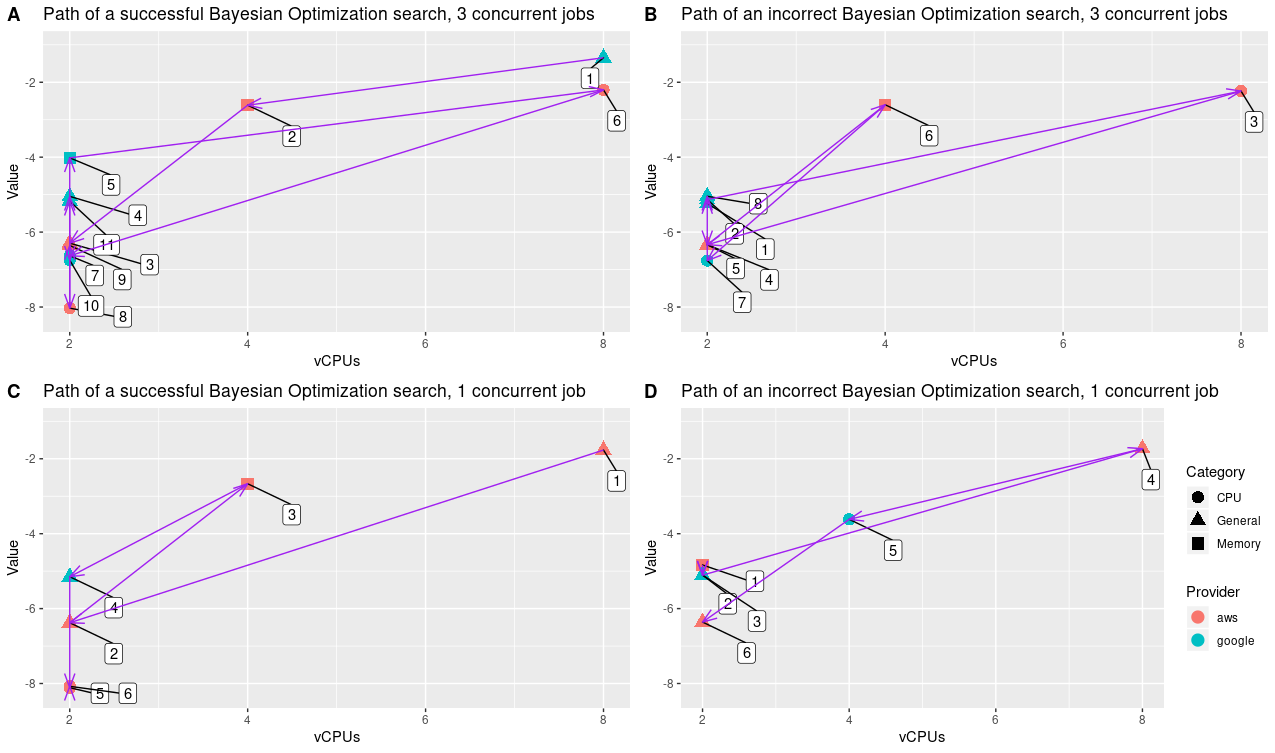
\includegraphics[scale=0.4]{paths}
	\caption{Paths of example Bayesian Optimization jobs}
	\label{fig:paths}
\end{figure}

\paragraph{}
With the exhaustive search complete, we then used a Spearmint based searcher to perform a Bayesian Optimization search, assuming low noise (-1 to 1) and using the same stopping conditions as used by default in the Cherrypick paper \cite{Alipourfard2017}, namely when the Expected improvement (EI) is less than 10\%, and at least 6 samples have been taken. We were able to successfully run this experiment with both multiple and single providers, as well as with between 1 and 3 multiple concurrent jobs. The results from these experiments are shown in figure \ref{fig:bo-results}, while examples of the job paths taken during them are shown in figure \ref{fig:paths}. Figure \ref{fig:bo-boxplots} shows the difference in values returned, time taken, and estimated search cost for different experiment configurations.


When testing instances from only a single provider, and running only a single concurrent job at any time, we were able to replicate the findings of the Cherrypick paper \cite{Alipourfard2017}. In 85\% of cases (17 of 20 experiments), Bayesian Optimization was able to reach the same conclusions as Exhaustive search in only 6-12 samples. 

Despite increasing the number of providers, with only a single concurrent job running, we were also able to replicate the previous results, with the correct optimal instance predicted in 18 out of 20 evaluations, in only 6-11 samples. For our evaluation, despite doubling the search space, Bayesian Optimization was no less effective.  It may be interesting to note, however, that the incorrectly predicted instance in both failed cases was not the second but third best choice, coming from the same provider rather than the other, resulting in a reduction in the mean score/cost value by ~21.3\%.  

By allowing 2 concurrent jobs to be run at any one time, the time taken for the search was reduced to less than half that of before ($P < .001$), without any significant loss in value returned ($P = .97$) or rise in search cost ($P = .79$). However, increasing the number of concurrent jobs higher, to 3, causes a dramatic reduction in effectiveness. The probability of returning a sub-optimal instance increases, while increasing the search cost compared to 2 concurrent jobs ($P = .024$) without any significant further decrease in search time ($P = .46$). To ensure this held true even in a reduced search space, the experiment was repeated with 3 concurrent jobs but only a single provider, to similar results.


\paragraph{}
Having performed evaluation on our implementation for a deployment of a simple docker container, effectively corresponding to running a single batch job or benchmark and interpreting the results, we then wanted to evaluate the same technique applied to an web-based application, which may be better evaluated through its responses to a client. For this a single 5-node Kubernetes cluster was set up for the same of sending repeated requests to the evaluated deployment, as described for the 'Pingserver' deployer and interpreter. This experiment is much more intensive to perform exhaustive search for, as it would require separate pinging clusters to be set up for every sample. The mean response time for requests of a normally distributed load was divided by the hourly cost of the instance to give maximised value. From the samples taken during 10 repetitions of this experiment, it seemed that there were no significant difference between the two optimal configurations of c5.large and m5.large ($\Delta \bar{x}=0.0001, P \approx 1.000$), which the predictions correctly converged upon in all cases.

\begin{figure}
  \caption{Values, search costs and times for different Bayesian Optimization searches. Single large outlier removed from search time graph from Single provider, 3 concurrent jobs.}
  \label{fig:bo-boxplots}
  \centering
  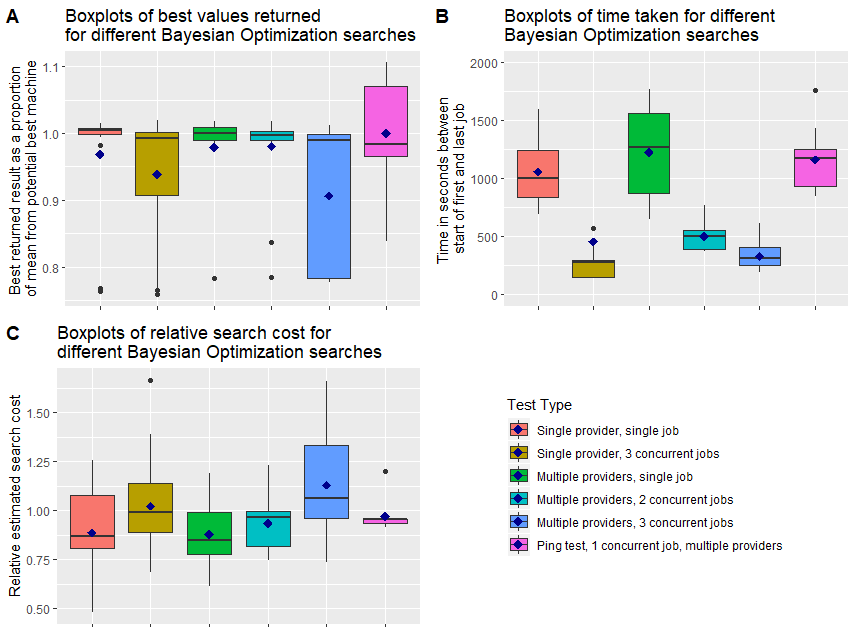
\includegraphics[scale=0.5]{bo_boxplots}
\end{figure}

\bibliographystyle{ieeetr}
\newpage
\bibliography{Dissertation}
\end{document}